% LaTeX Template for Project Report, Version 2.0
% (Abstracted from a Major Project Report at CSED, NIT Calicut but can be
% modified easily to use for other reports also.)
%
% Released under Creative Commons Attribution license (CC-BY)
% Info: http://creativecommons.org/licenses/by/3.0/
%
% Created by: Kartik Singhal
% BTech CSE Batch of 2009-13
% NIT Calicut
% Contact Info: kartiksinghal@gmail.com
%
% It is advisable to learn the basics of LaTeX before using this template.
% A good resource to start with is http://en.wikibooks.org/wiki/LaTeX/
%
% All template fields are marked with a pair of angular brackets e.g. <title here>
% except for the ones defining citation names in ref.tex.
%
% Empty space after chapter/section/subsection titles can be used to insert text.
%
% Just compile this file using pdflatex after making all required changes.

\documentclass[12pt,a4paper]{report}
\usepackage[toc,page]{appendix}
\usepackage[pdftex]{graphicx} %for embedding images
\usepackage{url} %for proper url entries
\usepackage{amsmath}
\usepackage[bookmarks, colorlinks=false, pdfborder={0 0 0}, pdftitle={<pdf title here>}, pdfauthor={<author's name here>}, pdfsubject={<subject here>}, pdfkeywords={<keywords here>}]{hyperref} %for creating links in the pdf version and other additional pdf attributes, no effect on the printed document
%\usepackage[final]{pdfpages} %for embedding another pdf, remove if not required

\begin{document}
\renewcommand\bibname{References} %Renames "Bibliography" to "References" on ref page

%include other pages
\begin{titlepage}
	
\begin{center}
		
\textup{\small {\bf MA308 Mini Project} \\ Report}\\[0.2in]
		
% Title
\Large \textbf {Designing a shortest-path algorithm for large-scale graphs}\\[0.2in]
\begin{center}
\small {Submitted in partial fulfillment of MA308 (Mini Project) requirements \\ III\textsuperscript{rd} Year / VI\textsuperscript{th} Semester - May 2025}
\end{center}

\includegraphics[width=1\textwidth]{./msc-logo}\\[0.1in]
		
		
% Submitted by
\normalsize Submitted by \\
\begin{table}[h]
\centering
\begin{tabular}{lr}\hline \\
Roll No. & Names of Students \\ \\ \hline
\\
I22MA023 & Abhinav Kumar \\ 
I22MA038 &  Raj Kumar \\
I22MA062 & Chandra Pratap \\ \\ \hline 
\end{tabular}
\end{table}
		
\vspace{.1in}
Under the guidance of\\
\large{\textbf{Dr. Sushil Kumar}}\\[0.2in]
		
\vfill
		
% Bottom of the page

\includegraphics[width=0.18\textwidth]{./svnit-logo}\\[0.1in]
\Large{Department of Mathematics}\\
\normalsize
\textsc{Sardar Vallabhbhai National Institute of Technology, Surat}\\
\vspace{0.2cm}
Even Semester 2024
		
\end{center}
	
\end{titlepage}
\documentclass[12pt]{article}

% Required packages
\usepackage{xcolor}     % For text color
\usepackage{geometry}   % For page margins
\usepackage{setspace}   % For spacing
\usepackage{ragged2e}   % For text alignment

% Page setup
\geometry{a4paper, margin=0.8in}
\setstretch{1.2}

\begin{document}
	
	% Centered blue heading
	\begin{center}
		{\color{blue} \Huge \textbf{Acknowledgments}}
	\end{center}
	
	\vspace{0.3cm}
	
	\justifying
	We, the students of the 5-Year Integrated M.Sc. in Mathematics program at Sardar Vallabhbhai National Institute of Technology, Surat take this opportunity to express our profound gratitude to everyone who supported and guided us throughout this mini-project.
	\vspace{0.2cm} 
	
	Our deepest thanks goes to \textbf{Dr. Sushil Kumar}, whose exceptional mentorship, guidance and encouragement have been pivotal to the success of this project. His ability to provide thoughtful insights and challenge us intellectually has greatly enriched our learning experience. Working under his supervision has been a rewarding and transformative experience that will benefit us throughout our academic and professional journeys.
	\vspace{0.2cm} 
	
	We are equally grateful to \textbf{Dr. Anupam Shukla}, Director of SVNIT Surat, and \textbf{Dr. Jayesh M. Dhodiya}, Head of the Department of Mathematics, for their leadership and support in fostering an environment that prioritizes academic excellence and research innovation. We also extend our gratitude to all the faculty members, research scholars, and non-teaching staff of the department for their valuable assistance, constant encouragement, and willingness to help whenever needed.
	\vspace{0.3cm} 
	
	This project was a collaborative effort, and we would like to acknowledge the contributions of one another, as well as those who supported us beyond the academic sphere:
	
	\vspace{0.3cm}
	
	I am deeply thankful to \textbf{Dr. Sushil Kumar} for his unwavering support, which has been instrumental in overcoming challenges during this project. I am grateful to my teammates for their cooperation and dedication, making this collaboration a fulfilling experience. Special thanks to my parents for their unconditional support and encouragement, as well as to all those who offered their assistance throughout this journey.
	
	\vspace{0.1cm} 
	\hfill \textbf{Abhinav Kumar} 
	
	\vspace{0.2cm} 
	
	I extend my sincere gratitude to \textbf{Dr. Sushil Kumar}, whose guidance has been crucial in shaping my understanding of this subject. His mentorship has made this project both insightful and rewarding. I am also immensely thankful to my teammates, \textbf{Abhinav Kumar} and \textbf{Chandra Pratap}, for their enthusiasm and teamwork. Finally, I wish to thank my family and friends for their encouragement, which has been a constant source of motivation during this project.
	
	\vspace{0.1cm} 
	\hfill \textbf{Raj Kumar} 
	
	\vspace{0.2cm} 
	
	I express my heartfelt gratitude to \textbf{Dr. Sushil Kumar}, whose support and expertise have been invaluable in the successful completion of this project. I am thankful to my teammates, \textbf{Abhinav Kumar} and \textbf{Raj Kumar}, for their dedication, without which this project would not have been possible. I also extend special thanks to \textbf{Harsh Mishra} and \textbf{Manish Raj} for their critical assistance in resolving a graph algorithm challenge, which was a turning point in our work. Lastly, I am grateful to my family and friends, whose encouragement, patience, and unwavering belief in my abilities have been a source of strength throughout this journey.
	
	\vspace{0.2cm} 
	\hfill \textbf{Chandra Pratap} 
	

\end{document}

\newpage
\thispagestyle{empty}

\begin{center}

\includegraphics[width=0.18\textwidth]{./svnit-logo}\\[0.1in]
\huge{Department of Mathematics}\\[0.1cm]
\normalsize
\textbf{\textsc{Sardar Vallabhbhai National Institute of Technology, Surat \\ SURAT-395007, GUJARAT, INDIA}}\\[1.5cm]
	
	
\textbf{\LARGE \underline{CERTIFICATE}}\\[0.5cm]
\end{center}
\normalsize This is to certify that this is a bonafide record of the project presented by the students whose names are given below during the even semester of 2024 in partial fulfilment of the requirements of the degree of Integrated Masters of Science in Mathematics.\\[1.0cm]

\begin{table}[h]
\centering
\begin{tabular}{lr}
Roll No & Names of Students \\ \\ \hline
\\
I22MA023 & Abhinav Kumar \\ 
I22MA038 &  Raj Kumar \\
I22MA062 & Chandra Pratap \\
\end{tabular}
\end{table}

\vfill

% Bottom of the page
\begin{flushright}
Dr. Sushil Kumar\\
(Project Guide)\\[1.5cm]
Dr. Ramakanta Meher\\
(Course Coordinator)\\
\end{flushright}

\begin{flushleft}
Date: 20 January, 2025
\end{flushleft}
\vspace{2in}
\chapter*{Abstract}

The proposed solution integrates traditional algorithms like Dijkstra’s and 
This project focuses on designing, implementing, and analyzing efficient algorithms for shortest path calculations on large-scale graphs, including social, road, and communication networks. The goal is to optimize computation time, memory usage, and scalability while ensuring high accuracy and adaptability to real-world scenarios.

The proposed solution combines traditional algorithms like Dijkstra’s and Bellman-Ford with advanced techniques such as A*, Contraction Hierarchies, and bidirectional search.

Publicly available datasets, including road networks from OpenStreetMap, are used to evaluate performance based on execution time, memory efficiency, and scalability.

Deliverables include a research report, an optimized algorithm codebase, a visualization tool for shortest path computations, performance analysis, and a discussion on strengths, limitations, and future improvements.



\pagenumbering{roman} %numbering before main content starts
\tableofcontents
\listoffigures

\newpage
\pagenumbering{arabic} %reset numbering to normal for the main content

\chapter{Problem Definition}

\section{Graph Representation}
	\begin{itemize}
		\item Define the graph G=(V, E) where V is the set of vertices (nodes) and E is the set of edges.
		\item Edge weights represent costs (e.g., travel time, distance, tolls).
	\end{itemize}
\section{Objectives}
	\begin{itemize}
		\item Minimize computation time for shortest path queries.
		\item Incorporate real-time edge weight updates.
		\item Allow customizable routing based on user-defined cost functions.
	\end{itemize}
 %objective changed to problem definition
\chapter{Introduction}

\title{Importance of Shortest Path Algorithm}

	\section{Importance of Sortest Path Calulation}
	\begin{itemize}
		\item \textbf{Efficiency in Large-Scale Systems}: In large graphs, such as road networks or the internet, finding an optimal route is essential to saving time, energy, and resources. These systems often involve millions of nodes and edges, requiring algorithms that handle complexity efficiently.
		\item \textbf{Optimization and Cost Reduction}: Many industries rely on shortest path calculations to minimize costs. For example, logistics companies use them to determine the most fuel-efficient routes for deliveries.
		\item \textbf{Road Networks and Navigation Systems}: GPS services like Google Maps calculate the shortest or fastest route to a destination based on real-time traffic data, distance, and road conditions.
		\item \textbf{Network Routing}: In computer networks, protocols like Open Shortest Path First (OSPF) or Border Gateway Protocol (BGP) rely on shortest path calculations to ensure efficient data transfer.
		\item \textbf{Social Network Analysis}: Platforms like LinkedIn or Facebook use these methods to determine the "degree of separation" between users or suggest connections.
	\end{itemize}
    \clearpage

	\section{Objective}
	The algorithm aims to:
	\begin{enumerate}
		\item \textbf{Accelerate shortest path queries}: The use of preprocessing optimizes search efficiency, enabling near-instantaneous path retrieval in large-scale networks.
		\item \textbf{Ensure scalability}: The algorithm is designed to handle extensive datasets, making it applicable to real-world scenarios, from urban traffic management to large-scale logistics planning.
	\end{enumerate}
	
	\section{Scope}
	This project is centered on developing a \textbf{hybrid shortest path algorithm} with a focus on the following key areas:
	\begin{itemize}
		\item \textbf{Road Networks}: The algorithm is specifically designed for road networks, where edge weights represent dynamic attributes such as travel time, distance, or toll fees. The approach ensures efficient routing solutions in real-world transportation systems.
		\item \textbf{Scalability and Efficiency}: Given the vast size of modern transportation and logistics networks, the algorithm must be capable of handling millions of nodes and edges while maintaining optimal performance.
		\item \textbf{Preprocessing for Speed Optimization}: Since traditional shortest path algorithms are computationally expensive, the project emphasizes the role of preprocessing in reducing query response times, ensuring rapid access to route data even in complex graphs.
	\end{itemize}

 %literature survey included in this
\chapter{Literature Review}
 In this chapter, we review the foundations and advanced algorithms for shortest path calculations, including preprocessing techniques. The section spans classical algorithms, advanced algorithms and recent advances in graph-optimization.
\section{Classical shortest path algorithms}
	\subsection{Breadth-first Search}
		\subsubsection{Introduction}
		Breadth-first search is a graph traversal algorithms invented by Konrad Zuse in 1945, that can also be used to find the shortest path from a source vertex to a destination vertex in an unweighted graph.
		
		\subsubsection{Algorithm}
			\begin{enumerate}
				\item Mark all vertices as unvisited.
				\item Assign $distance[u] = \infty$ for all vertices except the source vertex $s$, where $distance[s] = 0$.
				\item Use a queue to track vertices to explore. Start with the source vertex $s$.
				\item Dequeue a vertex $u$.
				\item For each neighbour $v$ of $u$, If $v$ is unvisited (i.e., $distance[v]=\infty$):
					\begin{itemize}
						\item Set $distance[v] = distance[u] + 1$.
						\item Mark $v$ as visited.
						\item Enqueue $v$.
					\end{itemize}
				\item The algorithm ends when the queue is empty. Unreachable vertices retain $distance = \infty$.
			\end{enumerate}
			This algorithm is mathematically predisposed to find the shortest path from a source vertex $s$ to every other vertex in the graph (see\textbf{ Appendix \ref{appendix:bfs:correctness}} for a formal proof).
		
		\subsubsection{Complexity}
			When finding the shortest path between a pair of vertices in a graph, the worst-case time complexity for the BFS algorithm is $O(V)$ for queue operations + $O(E)$ for edge processing, netting a worst-case time complexity of $O(V + E)$ (see \textbf{Appendix \ref{appendix:bfs:complexity}} for a formal proof). \medskip
			
			The space complexity for BFS is $O(V)$ since we use a queue to store the vertices yet to be explored.
		
		\subsubsection{Pros and Cons}
			\begin{itemize}
				\item The algorithm is simple and efficient for unweighted graphs.
				\item BFS works well for large, sparse graphs.
				\item BFS fails for shortest-path problems in weighted graphs, which are more useful when modelling real world scenarios.
			\end{itemize}
	\subsection{Bellman-ford Algorithm}
		\subsubsection{Introduction}
			The Bellman–Ford algorithm is a shortest-path algorithm that utilizes dynamic programming to compute shortest paths from a single source vertex to all of the other vertices in a weighted, directed graph. It was first published by Richard Bellman (1958) and Lester Ford Jr. (1956), hence its name.
		\subsubsection{Algorithm}
			\begin{enumerate}
				\item Create an array $distance$ of size $V$ to store the shortest path distances.
				\item Assign $distance[u] = \infty$ for all vertices except the source vertex $s$, where $distance[s] = 0$.
				\item Repeat $V - 1$ times:
					\begin{itemize}
						\item For each edge $(u,v) \in E$, if $distance[u] + w(u,v) < distance[v]$ update $distance[v]=distance[u]+w(u,v)$.
					\end{itemize}
				\item Now to detect a negative cycle, for each edge $(u,v) \in E$, if $distance[u] + w(u,v) < distance[v]$, report that a negative-weight cycle exists.
				\item If no negative-weight cycle is detected, Return the $distance$ array as the shortest path distances.
			\end{enumerate}
			Refer to \textbf{Appendix \ref{appendix:bellford:correctness}} for a formal proof of correctness of this algorithm.
		\subsubsection{Complexity}
			When finding the shortest path from a source vertex to every other vertex in a graph, the worst-case time complexity for the Bellman-Ford algorithm is $O(V \cdot E)$ (see \textbf{Appendix \ref{appendix:bellford:complexity}} for a formal proof). \medskip
			
			The space complexity for Bellman-Ford is $O(V)$ since we use an array of size $V$ to store all the shortest-path distances.
		\subsubsection{Pros and Cons}
			\begin{itemize}
				\item Suitable for applications requiring negative weight handling, in which case it can detect the existence of a negative cycle.
				\item The Bellman-Ford algorithm is more complex than Dijkstra's algorithm.
				\item Much slower compared to Dijkstra's algorithm.
			\end{itemize}
	\subsection{Dijkstra's Algorithm}
		\subsubsection{Introduction}
			Dijkstra's algorithm is a greedy algorithm used to find the shortest paths from a single source vertex to all other vertices in a weighted graph with non-negative edge weights. It was conceived by computer scientist Edsger W. Dijkstra in 1956 and published three years later.
		\subsubsection{Algorithm}
		\begin{enumerate}
			\item Create an array $distance$ of size $V$ to store the shortest path distances and a priority queue $Q$ containing all vertices, prioritized by $distance$.
			\item Assign $distance[u] = \infty$ for all vertices except the source vertex $s$, where $distance[s] = 0$.
			\item While $Q$ is not empty:
				\begin{itemize}
					\item Extract the vertex u u with the smallest distance distance from $Q$.
					\item For each neighbor $v$ of $u$, if $distance[u] + w(u,v) < distance[v]$: update $distance[v]=distance[u]+w(u,v)$ and the priority of $v$ in $Q$.
				\end{itemize}
			\item The algorithm ends when $Q$ is empty. The distance distance array contains the shortest path distances from $s$ to all other vertices.
		\end{enumerate}
			Refer to \textbf{Appendix \ref{appendix:dijkstra:correctness}} for a formal proof of correctness of this algorithm.
		\subsubsection{Complexity}
			When finding the shortest path from a source vertex to every other vertex in a graph, the worst-case time complexity for the Dijkstra's algorithm is $O((V+E)\log{V})$ using a binary heap or $O(V\log{V}+E)$ using a Fibonacci heap. (see \textbf{Appendix \ref{appendix:dijkstra:complexity}} for a formal proof). \medskip
			
			The space complexity for Dijkstra's is $O(V)$ since we use an array of size $V$ to store all the shortest-path distances.
		\subsubsection{Pros and Cons}
		\begin{itemize}
			\item Can cover a large area of a graph, which is useful when there are multiple target nodes.
			\item Can't calculate the shortest paths correctly if the graph has negative weights.
			\item Has linearithmetic complexity when implemented using a priority queue.
		\end{itemize}

\section{Advanced shortest path algorithms}
	\subsection{A* Search Algorithm}
		\subsubsection{Introduction}
			A* search is a heuristic-based algorithm used to find the shortest path from a start node to a goal node in a weighted graph. It combines the strengths of Dijkstra's algorithm (guaranteed shortest path) and greedy best-first search (efficient exploration using heuristics). It was first published by Peter Hart, Nils Nilsson, and Bertram Raphael at Stanford Research Institute in 1968.
		\subsubsection{Algorithm}
			\begin{enumerate}
				\item Create a priority queue $Q$ to store nodes to explore, prioritized by $f(v)=g(v)+h(v)$, where
					\begin{itemize}
						\item $g(v)$: Cost of the shortest path from $s$ to $v$ found so far.
						\item $h(v)$: Heuristic estimate of the cost from $v$ to $t$.
					\end{itemize}
				\item Set $g(s)=0$ and $f(s)=h(s)$.
				\item Insert $s$ into $Q$.
				\item Create a set $visited$ to track visited nodes
				\item While $Q$ is not empty:
					\begin{enumerate}
						\item Extract the node $u$ with the smallest $f(u)$ from $Q$.
						\item If $u=t$, return the path from $s$ to $t$.
						\item Mark $u$ as visited.
						\item For each neighbor $v$ of $u$, if $v$ is not visited:
							\begin{itemize}
								\item Compute $g_{tentative} = g(u) + w(u,v)$.
								\item If $g_{tentative} < g(v)$ or $v$ is not in $Q$:
									\begin{itemize}
										\item Update $g(v)=g_{tentative}$.
										\item Update $f(v)=g(v)+h(v)$.
										\item Insert $v$ into $Q$ (or update its priority if already in $Q$).
									\end{itemize}
							\end{itemize}
					\end{enumerate}
				\item If $Q$ becomes empty and the goal $t$ has not been reached, no path exists.
			\end{enumerate}
			A* search is correct if the heuristic $h(v)$ is admissible (never overestimates the true cost to the goal) and consistent (satisfies the triangle inequality: $h(u) \leq w(u,v)+h(v)$ for all edges $(u,v))$. For a formal proof of correctness, refer to \textbf{Appendix \ref{appendix:astar:correctness}}.
		\subsubsection{Complexity}
		Since A* Search is basically an 'informed' version of Dijkstra's algorithm, the space complexity for A* search is the same as for Dijkstra's, which is $O(V)$.
		The time complexity, however, depends on the heuristic function and is equal to Dijsktra's when the heuristic $h(v) = 0$.
		\subsubsection{Pros and Cons}
			\begin{itemize}
				\item Compared to uninformed search algorithms, A* explores significantly fewer nodes leading to faster search times. 
				\item By maintaining a priority queue, A* only needs to store a limited number of nodes in memory, making it suitable for large search spaces.
				\item Performance heavily depends on the quality of the heuristic function. Thus, A* search is not ideal when a good heuristic cannot be easily defined or when heuristic calculations are complicated.
			\end{itemize}
	\subsection{Bidirectional Search}
		\subsubsection{Introduction}
		\subsubsection{Algorithm}
		\subsubsection{Complexity}
		\subsubsection{Pros and Cons}
\section{Preprocessing techniques}
\subsection{Contraction Hierarchies}









%-----------------------------------------------------------------------------------------------------------------------------------------------------------------------------------

	\subsection{A* Landmark Technique  Algorithm}

		\subsubsection{Introduction}
		
			The ALT algorithm is a goal-directed search proposed by Golberg and Harrelson that uses the A* search algorithm and distance estimates to define node potentials that direct the search towards the target.
			It is a variant of the \textbf{A*} search algorithm where \textbf{L}andmarks and the \textbf{T}riangle inequality are used to compute for a feasible potential function. 

				\subsubsection{Algorithm}
						
				The ALT algorithm consists of two main phases:
				\subsubsection{Preprocessing Phase - Offline Computation}
				In this phase, ALT selects a set of \textit{landmarks} and precomputes the shortest distances from these landmarks to all nodes in the graph.
				
				\subsubsection{Step 1: Landmark Selection}
				\begin{itemize}
					\item Choose a set of landmarks $ \textit{L} $ (typically high-degree or far-apart nodes).
					\item Selection strategies:
					\begin{itemize}
						\item Select landmarks that maximize the shortest path distances between them.
						\item Choose nodes with high connectivity.
						\item Select a diverse set of nodes.
						
					\end{itemize}
				\end{itemize}
				
				\subsubsection{Step 2: Compute Shortest Path Distances from Landmarks}
				\begin{itemize}
					\item For each landmark $ L \in \textit{L} $, compute the shortest paths to \textit{all other nodes} in the graph using Dijkstra’s Algorithm.
					\item Store the \textit{precomputed distances} $ d(L, v) $ for every node $ v $
					\item If we have $ k $ landmarks and $ |V| $ nodes, we store $ O(k |V|) $ distances.
				\end{itemize}
				
				\subsubsection{Query Phase - Online Computation}
				When computing the shortest path from a source $ s $ to a target $ t $, ALT modifies \textit{A* search} by using a heuristic based on \textit{landmark distances}.
				
				\subsubsection{Step 1: Compute Heuristic Function}
				A* search requires a heuristic function $ h(v) $ that estimates the shortest distance from a node $ v $ to the target $ t $. ALT uses the \textit{triangle inequality} to define the heuristic.
				
					The heuristic function is defined as:
					
					\begin{equation}
						h(v) = \max_{L \in \textit{L}} \left( \left| d(L, v) - d(L, t) \right| \right)
					\end{equation}
					
					where:
					\begin{itemize}
						\item \textit{L}  is the set of selected \textit{landmarks}
						
						\item $ d(L, v) $ is the precomputed shortest distance from landmark $ L $ to node $ v $
						
						\item $ d(L, t) $ is the precomputed shortest distance from landmark $ L $ to the target $ t $.
					\end{itemize}
				
				\subsubsection{Step 2: Run A* Search with ALT Heuristic}
				\begin{itemize}
					\item Initialize A* search from source $ s $ to target $ t $.
					\item Instead of using a simple heuristic (e.g., Euclidean distance), use the \textit{ALT heuristic}  $ h(v) $.
					\item Expand nodes in order of their priority, defined by:
					
					\begin{equation}
					f(v) = g(v) + h(v)
					\end{equation}
					
					where:
					\begin{itemize}
						\item $ g(v) $ is the actual distance from $ s $ to $ v $ (computed dynamically).
						\item $ h(v) $ is the ALT heuristic (precomputed from landmarks).
					\end{itemize}
					\item Since $ h(v) $ is \textit{admissible} (never overestimates the true distance), ALT guarantees an \textit{optimal shortest path}.
				\end{itemize}
				
				\subsubsection{Step 3: Termination}
				\begin{itemize}
					\item A* terminates when the target $ t $ is dequeued (meaning the shortest path has been found).
					\item The total cost of the path is stored in $ g(t) $.
				\end{itemize}

			This algorithm is mathematically predisposed to find the shortest path from a source vertex $s$ to every other vertex in the graph 
			
			Refer \textbf{ Appendix \ref{appendix:ALT:correctness}} for the formal proof.
			

		\subsubsection{Complexity}

				\begin{itemize}
					\item \textbf{Preprocessing Time Complexity:} $ O(k \cdot (|V| + |E|) \log |V|) $
					\item \textbf{Query Time Complexity:} $ O((|V| + |E|) \log |V|) $  (in the worst case)
					\item \textbf{Space Complexity:} $ O(k \cdot |V|) $
				\end{itemize}


				Refer \textbf{Appendix \ref{appendix:ALT:complexity}} for the formal proof. \medskip
				
		\subsubsection{Pros and Cons}
		\begin{itemize}
			\item Precomputed landmarks and A* heuristics speed up shortest path searches.
			\item Significant preprocessing time and memory usage.
			\item Properly chosen landmarks enhance performance, but poor selection can degrade efficiency, affecting search quality.
			\item Inefficient for frequently changing networks
		\end{itemize}



%-----------------------------------------------------------------------------------------------------------------------------------------------------------------------------------

	\subsection{Hub Labeling}

		\subsubsection{Introduction}
		Hub Labeling (HL) is a preprocessing-based technique for efficient shortest path queries in graphs. It assigns labels to nodes, storing distances to selected hubs, enabling constant-time distance queries.
		
			\subsubsection{Algorithm}

				Let $ G = (V, E) $ be a graph where $ V $ is the set of vertices and $ E $ is the set of edges.
				
			\subsubsection{Step 1: Preprocessing Phase}
				\begin{itemize}
					\item \textit{Hub Selection:}  
					Select a subset \( H \subseteq V \) of \( k \) nodes as hubs, based on heuristics such as high-degree nodes or random selection.
				
					\item \textit{Compute Shortest Paths:}  
						\begin{itemize}
						
						\item For each $ v \in V $, compute the shortest path distances to each hub $ h \in H $, i.e., $ d(v, h) $, using Dijkstra’s algorithm or another shortest path algorithm.  
						
						\item Store the distances in the hub label of node $ v $, denoted as:
						$
						L(v) = \{ d(v, h) \mid h \in H \}
						$
						
						\item The preprocessing time complexity is:
						$
						O(k \cdot (|V| + |E|) \log |V|)
						$
						where $ k $ is the number of hubs.
						
						\end{itemize}
					\end{itemize}
			\subsubsection{Step 2: Query Phase}
				
				Given a query between nodes $ s $ and $ t $, the shortest path $ d(s, t) $ can be computed as:
				
						\begin{equation}
							d(s,t) = \min_{h \in H} \left( d(s,h) + d(h,t) \right)
						\end{equation}


				where:
				
				\begin{itemize}
					\item $ d(s, h) $ is the distance from $ s $ to hub $ h $,
					\item $ d(h, t) $ is the distance from hub $ h $ to $ t $.
				\end{itemize}
				
			
			
			Refer \textbf{Appendix \ref{appendix:Hub Labelling:correctness}} for the formal proof.
			
				\subsubsection{Complexity}
					\begin{itemize}
						\item \textit{Preprocessing Time Complexity:}  $ O(k \cdot (|V| + |E|) \log |V|) $
						\item \textit{Query Time Complexity:}  $ O(k) $
						\item \textit{Space Complexity:}  $ O(k \cdot |V|) $
					\end{itemize} 
	
			Refer \textbf{Appendix \ref{appendix:Hub Labelling:Complexity}} for the formal proof. 
				
				\subsubsection{Pros and Cons}
				\begin{itemize}
					\item Precomputed hub labels enable constant-time shortest path lookups.
					\item Building hub labels requires extensive computation and storage.
					\item Works well for large static graphs but demands significant memory.
					\item Frequent updates require costly recomputation.
				\end{itemize}
										
				

%-----------------------------------------------------------------------------------------------------------------------------------------------------------------------------------


% Refer figure \ref{fig:label}.

\section{Summary of Findings}
%\begin{figure}[htb]
%\centering
%
\includegraphics[scale=0.3]{./glider} % e.g. insert ./image for image.png in the working directory, adjust scale as necessary
%\caption{Caption here}
%\label{fig:label} % insert suitable label, this is used to refer to a fig from within the text as shown above
%\end{figure}


\chapter{Algorithm Design}

\section{Preprocessing Phase}
	\begin{itemize}
		\item Explain the choice of preprocessing techniques (e.g., Contraction Hierarchies, ALT).
		\item Describe how the graph is simplified or augmented with shortcuts/landmarks.
		\item Discuss trade-offs in preprocessing time and memory usage.
	\end{itemize}
\section{Query Execution}
	\begin{itemize}
		\item Detail the hybrid algorithm combining preprocessing results with A* or bidirectional search.
		\item Include pseudocode for the query phase.
	\end{itemize}
\section{Dynamic Updates}
	\begin{itemize}
		\item Describe methods for updating edge weights and recalculating shortest paths efficiently.
		\item Outline incremental update mechanisms.
	\end{itemize}
\section{Customization}
	\begin{itemize}
		\item Define the composite cost function and how it integrates with the algorithm.
	\end{itemize}
\chapter{Implementation}

\section{Implementation Details}

\subsection{Key Python Files}
\begin{itemize}
	\item \texttt{algorithms.py} – Contains the core logic and pathfinding algorithms such as Dijkstra, A*, Bidirectional Dijkstra, Bidirectional A*, ALT, and Bidirectional ALT.
	\item \texttt{animation.py} – Handles the visual output and animation of the pathfinding process using map data.
	\item \texttt{pathfinder.py} – The main script that integrates the algorithms and visualization. It performs graph generation, pathfinding, and animation.
	\item \texttt{test.py} – Used for testing the functionality and accuracy of implemented algorithms.
\end{itemize}

\subsection{Libraries Used}
\begin{itemize}
	\item \textbf{osmnx}: A Python package used to download and work with real-world street networks from OpenStreetMap. It is utilized for generating graphs of city maps and identifying nodes based on geographic coordinates. Key functions used include \texttt{graph\_from\_bbox} and \texttt{nearest\_nodes}.
	
	\item \textbf{Custom Modules}:
	\begin{itemize}
		\item \texttt{animation.py} – Handles visualization and animation of pathfinding algorithms.
		\item \texttt{algorithms.py} – Contains implementations of Dijkstra, A*, Bidirectional A*, ALT Preprocessing, and Bidirectional ALT algorithms.
	\end{itemize}
\end{itemize}

\subsection{Graph Generation and Pathfinding}
The implementation uses \texttt{osmnx} to fetch map data of a specific region in Surat, bounded around SVNIT and Surat Railway Station. The graph is created using a bounding box, and the start and end points are mapped to the closest nodes in the graph using their latitude and longitude coordinates.

\begin{lstlisting}[language=Python, caption={Pathfinding and Animation Code}, label={lst:pathfinding}]
	import osmnx as ox
	from animation import Animator
	from algorithms import dijkstra, bidirectional_alt_query, ALTPreprocessor
	
	# Load map data of Surat
	G = ox.graph_from_bbox(72.75, 72.87, 21.13, 21.22)
	
	# Define start and end nodes (SVNIT to Surat Railway Station)
	start_node = ox.distance.nearest_nodes(G, 72.7865, 21.1634)
	end_node = ox.distance.nearest_nodes(G, 72.8410, 21.2055)
	
	animator = Animator(G, start_node, end_node, ALTPreprocessor(G))
	animator.animate_path(bidirectional_alt_query)
\end{lstlisting}


The above code demonstrates the following:
\begin{itemize}
	\item \textbf{Graph Creation}: A real-world street network graph of Surat is created using \texttt{osmnx}.
	\item \textbf{Node Selection}: Start and end locations are converted into graph nodes using geographic coordinates.
	\item \textbf{Pathfinding Algorithms}: Shortest paths are calculated using both Dijkstra’s algorithm and Bidirectional ALT (A*, Landmarks, Triangle inequality).
	
	\item \textbf{Visualization}: An animation is created using the \texttt{Animator} class to dynamically visualize the pathfinding process.
\end{itemize}


\section*{Algorithm Implementations and Details}

\subsection*{Libraries Used}
\begin{itemize}
	\item \textbf{heapq} -- Efficient priority queue used for all algorithms.
	\item \textbf{math} -- Supports mathematical calculations for heuristics in A* and ALT.
	\item \textbf{networkx} -- Handles graph operations such as neighbor access and edge data.
\end{itemize}

\subsection*{1. Dijkstra's Algorithm}
\begin{lstlisting}[language=Python, caption=Classical Dijkstra’s Algorithm]
	def dijkstra(graph, start, end):
	visited_edges, optimal_path = [], []
	
	queue = []
	heapq.heappush(queue, (0, start, [start]))
	
	shortest_distance = {node: float('inf') for node in graph.nodes}
	shortest_distance[start] = 0
	
	while queue:
	current_cost, current_node, current_path = heapq.heappop(queue)
	if current_cost > shortest_distance[current_node]:
	continue
	
	if current_node == end:
	optimal_path = current_path
	break
	
	for neighbor in graph.neighbors(current_node):
	edge_costs = [data.get('length', 1) for data in graph[current_node][neighbor].values()]
	min_edge_cost = min(edge_costs)
	total_cost = current_cost + min_edge_cost
	
	if total_cost < shortest_distance[neighbor]:
	shortest_distance[neighbor] = total_cost
	heapq.heappush(queue, (total_cost, neighbor, current_path + [neighbor]))
	visited_edges.append((current_node, neighbor))
	
	return visited_edges, optimal_path
\end{lstlisting}

\subsubsection*{Explanation}
\begin{itemize}
	\item Classic shortest path algorithm, no heuristics involved.
	\item Uses a priority queue to explore the cheapest path to each node.
	\item Guarantees the optimal path in graphs with non-negative edge weights.
\end{itemize}

\subsection*{2. A* Search Algorithm}
\begin{lstlisting}[language=Python, caption=A* Search with Heuristic]
	def astar(graph, start, end):
	def heuristic(u, v):
	coord_u = graph.nodes[u]['x'], graph.nodes[u]['y']
	coord_v = graph.nodes[v]['x'], graph.nodes[v]['y']
	return ((coord_u[0] - coord_v[0]) ** 2 + (coord_u[1] - coord_v[1]) ** 2) ** 0.5
	
	visited_edges = []
	queue = [(0, start, [start])]
	shortest_distance = {node: float('inf') for node in graph.nodes}
	shortest_distance[start] = 0
	
	while queue:
	current_cost, current_node, path = heapq.heappop(queue)
	if current_node == end:
	return visited_edges, path
	
	for neighbor in graph.neighbors(current_node):
	cost = graph[current_node][neighbor][0].get('length', 1)
	total_cost = shortest_distance[current_node] + cost
	
	if total_cost < shortest_distance[neighbor]:
	shortest_distance[neighbor] = total_cost
	priority = total_cost + heuristic(neighbor, end)
	heapq.heappush(queue, (priority, neighbor, path + [neighbor]))
	visited_edges.append((current_node, neighbor))
\end{lstlisting}

\subsubsection*{Explanation}
\begin{itemize}
	\item Uses Euclidean distance as a heuristic to guide search.
	\item Reduces explored nodes compared to Dijkstra.
	\item Efficient for spatial graphs.
\end{itemize}

\subsection*{3. Bidirectional Dijkstra's Algorithm}
\begin{lstlisting}[language=Python, caption=Bidirectional Dijkstra's Algorithm]
	def bidirectional_dijkstra(graph, start, end):
	visited_edges = []
	
	forward_queue = [(0, start)]
	backward_queue = [(0, end)]
	
	shortest_distance_forward = {node: float('inf') for node in graph.nodes}
	shortest_distance_backward = {node: float('inf') for node in graph.nodes}
	shortest_distance_forward[start] = 0
	shortest_distance_backward[end] = 0
	
	best_total_cost = float('inf')
	meeting_node = None
	
	while forward_queue or backward_queue:
	process_forward = (
	not backward_queue or
	(forward_queue and forward_queue[0][0] <= backward_queue[0][0])
	)
	
	if process_forward:
	current_cost, current_node = heapq.heappop(forward_queue)
	for neighbor in graph.neighbors(current_node):
	pass  # Update forward distances
	else:
	current_cost, current_node = heapq.heappop(backward_queue)
	for neighbor in graph.neighbors(current_node):
	pass  # Update backward distances
	
	if shortest_distance_backward[current_node] != float('inf'):
	total_cost = current_cost + shortest_distance_backward[current_node]
	if total_cost < best_total_cost:
	best_total_cost = total_cost
	meeting_node = current_node
	
	return visited_edges, optimal_path
\end{lstlisting}

\subsubsection*{Explanation}
\begin{itemize}
	\item Simultaneously searches from start and end nodes.
	\item Reduces search space significantly.
	\item Merges paths at the meeting node for optimal path.
\end{itemize}



\subsection*{4. Bidirectional A* Algorithm}
\begin{lstlisting}[language=Python, caption=Bidirectional A* Search]
	def bidirectional_astar(graph, start, end):
	def heuristic(u, v):
	coord_u = graph.nodes[u]['x'], graph.nodes[u]['y']
	coord_v = graph.nodes[v]['x'], graph.nodes[v]['y']
	return ((coord_u[0] - coord_v[0]) ** 2 + (coord_u[1] - coord_v[1]) ** 2) ** 0.5
	
	forward_queue = [(heuristic(start, end), start)]
	backward_queue = [(heuristic(end, start), end)]
	
	# Similar to bidirectional Dijkstra with heuristics...
	
	return visited_edges, optimal_path
\end{lstlisting}

\subsubsection*{Explanation}
\begin{itemize}
	\item Combines bidirectional search with A* heuristic.
	\item Highly efficient for large graphs.
\end{itemize}

\subsection*{5. Bidirectional ALT Algorithm}
\begin{lstlisting}[language=Python, caption=ALT Preprocessing for Heuristics]
	class ALTPreprocessor:
	def __init__(self, graph):
	self.landmarks = self.select_landmarks(graph, 4)
	self.distances = self.compute_distances(graph)
	
	def select_landmarks(self, graph, count):
	return random.sample(list(graph.nodes), count)
	
	def compute_distances(self, graph):
	return {lm: nx.single_source_dijkstra_path_length(graph, lm) for lm in self.landmarks}
	
	def heuristic(self, u, v):
	estimates = [abs(self.distances[lm][u] - self.distances[lm][v]) for lm in self.landmarks]
	return max(estimates)

	def bidirectional_alt_query(graph, start, end, alt_preprocessor):
	visited_edges = []
	forward_queue = [(0, start, [start])]
	backward_queue = [(0, end, [end])]
	
	# Initialize distances and queues similar to bidirectional A*
	# Use alt_preprocessor.heuristic(u, v) in both directions
	
	return visited_edges, optimal_path
\end{lstlisting}

\subsubsection*{Explanation}
\begin{itemize}
	\item Landmarks are used to compute preprocessed distance estimates.
	\item Heuristic improves pathfinding performance.
	\item Combines bidirectional search with ALT heuristic.
	\item Reduces computation time and search space.
\end{itemize}



\section*{Animation Module – \texttt{animation.py}}

\subsection*{Libraries Used}
\begin{itemize}
	\item \textbf{pygame}: Used for creating real-time graphical animations of pathfinding algorithms.
	\item \textbf{cv2 (OpenCV)}: Likely used for video export features (used in other parts of the file).
	\item \textbf{numpy}: For numerical computations.
	\item \textbf{time}: To measure execution and animation durations.
\end{itemize}

\subsection*{Implementation Overview}
The \texttt{Animator} class is responsible for visualizing the execution of various pathfinding algorithms on a real-world map using Pygame. It supports:
\begin{itemize}
	\item Interactive animation of pathfinding steps.
	\item Preprocessing visualization if ALT (landmark-based) algorithms are used.
	\item Real-time mapping from geo-coordinates to screen pixels.
\end{itemize}

\begin{lstlisting}[language=Python, caption=Core logic of Animator class]
	import pygame
	import time
	import cv2
	import numpy as np
	
	class Animator:
	def __init__(self, graph, start, end, preprocessor=None):
	self.G = graph
	self.start_node, self.end_node = start, end
	self.preprocessor = preprocessor
	
	def _common_setup(self, algorithm):
	if self.preprocessor:
	start_preprocess = time.time()
	self.preprocessor._select_landmarks()
	self.preprocessor._precompute_distances()
	preprocessing_time = time.time() - start_preprocess
	
	algo_start = time.time()
	visited_edges, optimal_path = algorithm(
	self.G, self.start_node, self.end_node,
	*([self.preprocessor] if self.preprocessor else [])
	)
	algo_time = time.time() - algo_start
	
	# Coordinate normalization for screen rendering
	nodes = list(self.G.nodes(data=True))
	xs = [data['x'] for _, data in nodes]
	ys = [data['y'] for _, data in nodes]
	min_x, max_x, min_y, max_y = min(xs), max(xs), min(ys), max(ys)
	
	screen_width, screen_height = 1280, 720
	node_pos = {
		node: (
		int((data['x'] - min_x) / (max_x - min_x) * screen_width),
		int((1 - (data['y'] - min_y) / (max_y - min_y)) * screen_height)
		)
		for node, data in nodes
	}
	
	# Convert visited edges and optimal path to screen coordinates
	visited_edges_screen = [(node_pos[u], node_pos[v]) for u, v in visited_edges]
	optimal_path_edges_screen = [
	(node_pos[optimal_path[i]], node_pos[optimal_path[i + 1]])
	for i in range(len(optimal_path) - 1)
	]
	
	return visited_edges_screen, optimal_path_edges_screen
\end{lstlisting}
The class begins by initializing with a graph and node data. The method \texttt{\_common\_setup()} performs the following tasks:
\begin{itemize}
	\item \textbf{Preprocessing:} Landmark selection and distance matrix computation if the ALT (A* with Landmarks and Triangle inequality) method is used.
	\item \textbf{Algorithm Execution:} Executes the selected pathfinding algorithm and measures execution time.
	\item \textbf{Normalization:} Geo-coordinates from OpenStreetMap are normalized to fit a fixed screen resolution for display.
	\item \textbf{Rendering Data:} Converts visited edges and the optimal path into screen coordinates, preparing for graphical animation.
\end{itemize}
\chapter{Result and Analysis}
	To evaluate the performance of our various algorithm implementations, we use Python's \texttt{timeit} module to measure the execution time of both the standard \texttt{NetworkX.shortest\_path()} function and our custom algorithm. The following code demonstrates our approach:
	
	\begin{lstlisting}
		timer = timeit.Timer(lambda: nx.shortest_path(G, start_node, end_node))
		nx_time = min(timer.repeat(5, 100))
		print("NetworkX time:", nx_time)
		
		timer = timeit.Timer(lambda: algorithm(G, start_node, end_node, preprocessor))
		algo_time = min(timer.repeat(5, 100))
		print("Algorithm time:", algo_time)
		
		print(f"NetworkX's algorithm takes {nx_time / algo_time:.4%} of Algorithm's time")
	\end{lstlisting}
	
	This code operates as follows:
	\begin{enumerate}
		\item \textbf{Timing Setup:}  
		\begin{itemize}
			\item We create a \texttt{Timer} object from the \texttt{timeit} module with a lambda function that calls either \texttt{nx.shortest\_path(G, start\_node, end\_node)} or our custom \texttt{algorithm(G, start\_node, end\_node, preprocessor)}.
		\end{itemize}
		\item \textbf{Repeating the Measurement:}  
		\begin{itemize}
			\item The method \texttt{repeat(5, 100)} executes the lambda 100 times per iteration, repeated over 5 iterations. This returns a list of execution times.
		\end{itemize}
		\item \textbf{Selecting the Best Time:}  
		\begin{itemize}
			\item Instead of averaging the results, we use \texttt{min()} to select the lowest execution time. This minimum value represents a lower bound of the runtime under optimal conditions. Variability due to system load or background processes typically results in higher values, so using the minimum helps mitigate these effects.
		\end{itemize}
		\item \textbf{Performance Comparison:}  
		\begin{itemize}
			\item Finally, we compare the performance by printing the ratio of \texttt{nx\_time} to \texttt{algo\_time}. This ratio indicates how much faster (or slower) our custom algorithm is relative to NetworkX's implementation.
		\end{itemize}
	\end{enumerate}
	
	By timing both the standard and custom implementations in this way, we ensure a system-independent baseline for performance, making it possible to assess the inherent efficiency of our algorithm.

	 \section{Version 1: Basic Dijkstra's Algorithm}
	 	Running the timing code on this version produced the following output:
	 	\begin{verbatim}
	 		NetworkX time:  0.6769123002886772
	 		Algorithm time:  21.229514400009066
	 		NetworkX's algorithm takes 3.1885% of Algorithm's time
	 	\end{verbatim}
	 	While not optimal, this version serves as a valuable baseline for comparing subsequent, more advanced versions.

	 \section{Version 2: A* Search Algorithm}
	 	Running the timing code on this version produced the following output:
	 	\begin{verbatim}
			NetworkX time:  0.7038580998778343
			Algorithm time:  19.783792700152844
			NetworkX's algorithm takes 3.5578% of Algorithm's time
	 	\end{verbatim}
	 	
	 	This represents a \(\frac{3.5578}{3.1885} \approx 1.11\times\) improvement in execution time compared to Version 1. \newline
	 	
	 	Such a performance gain is consistent with the theoretical benefits of the A* algorithm, where a simple heuristic helps prioritize the exploration of nearer edges. As the size of the graph increases, we expect this improvement to become even more pronounced.
	 
	 \section{Version 3: Bidirectional Dijkstra's Algorithm}
	 	Running the timing code on this version produced the following output:
	 	\begin{verbatim}
	 		NetworkX time:  0.6851798999123275
	 		Algorithm time:  16.339504099916667
	 		NetworkX's algorithm takes 4.1934% of Algorithm's time
	 	\end{verbatim}
	 
		 This represents a \(\frac{4.1934}{3.5578} \approx 1.18\times\) improvement over Version 2. 
		 
		 \begin{figure}[H]
		 	\centering
		 	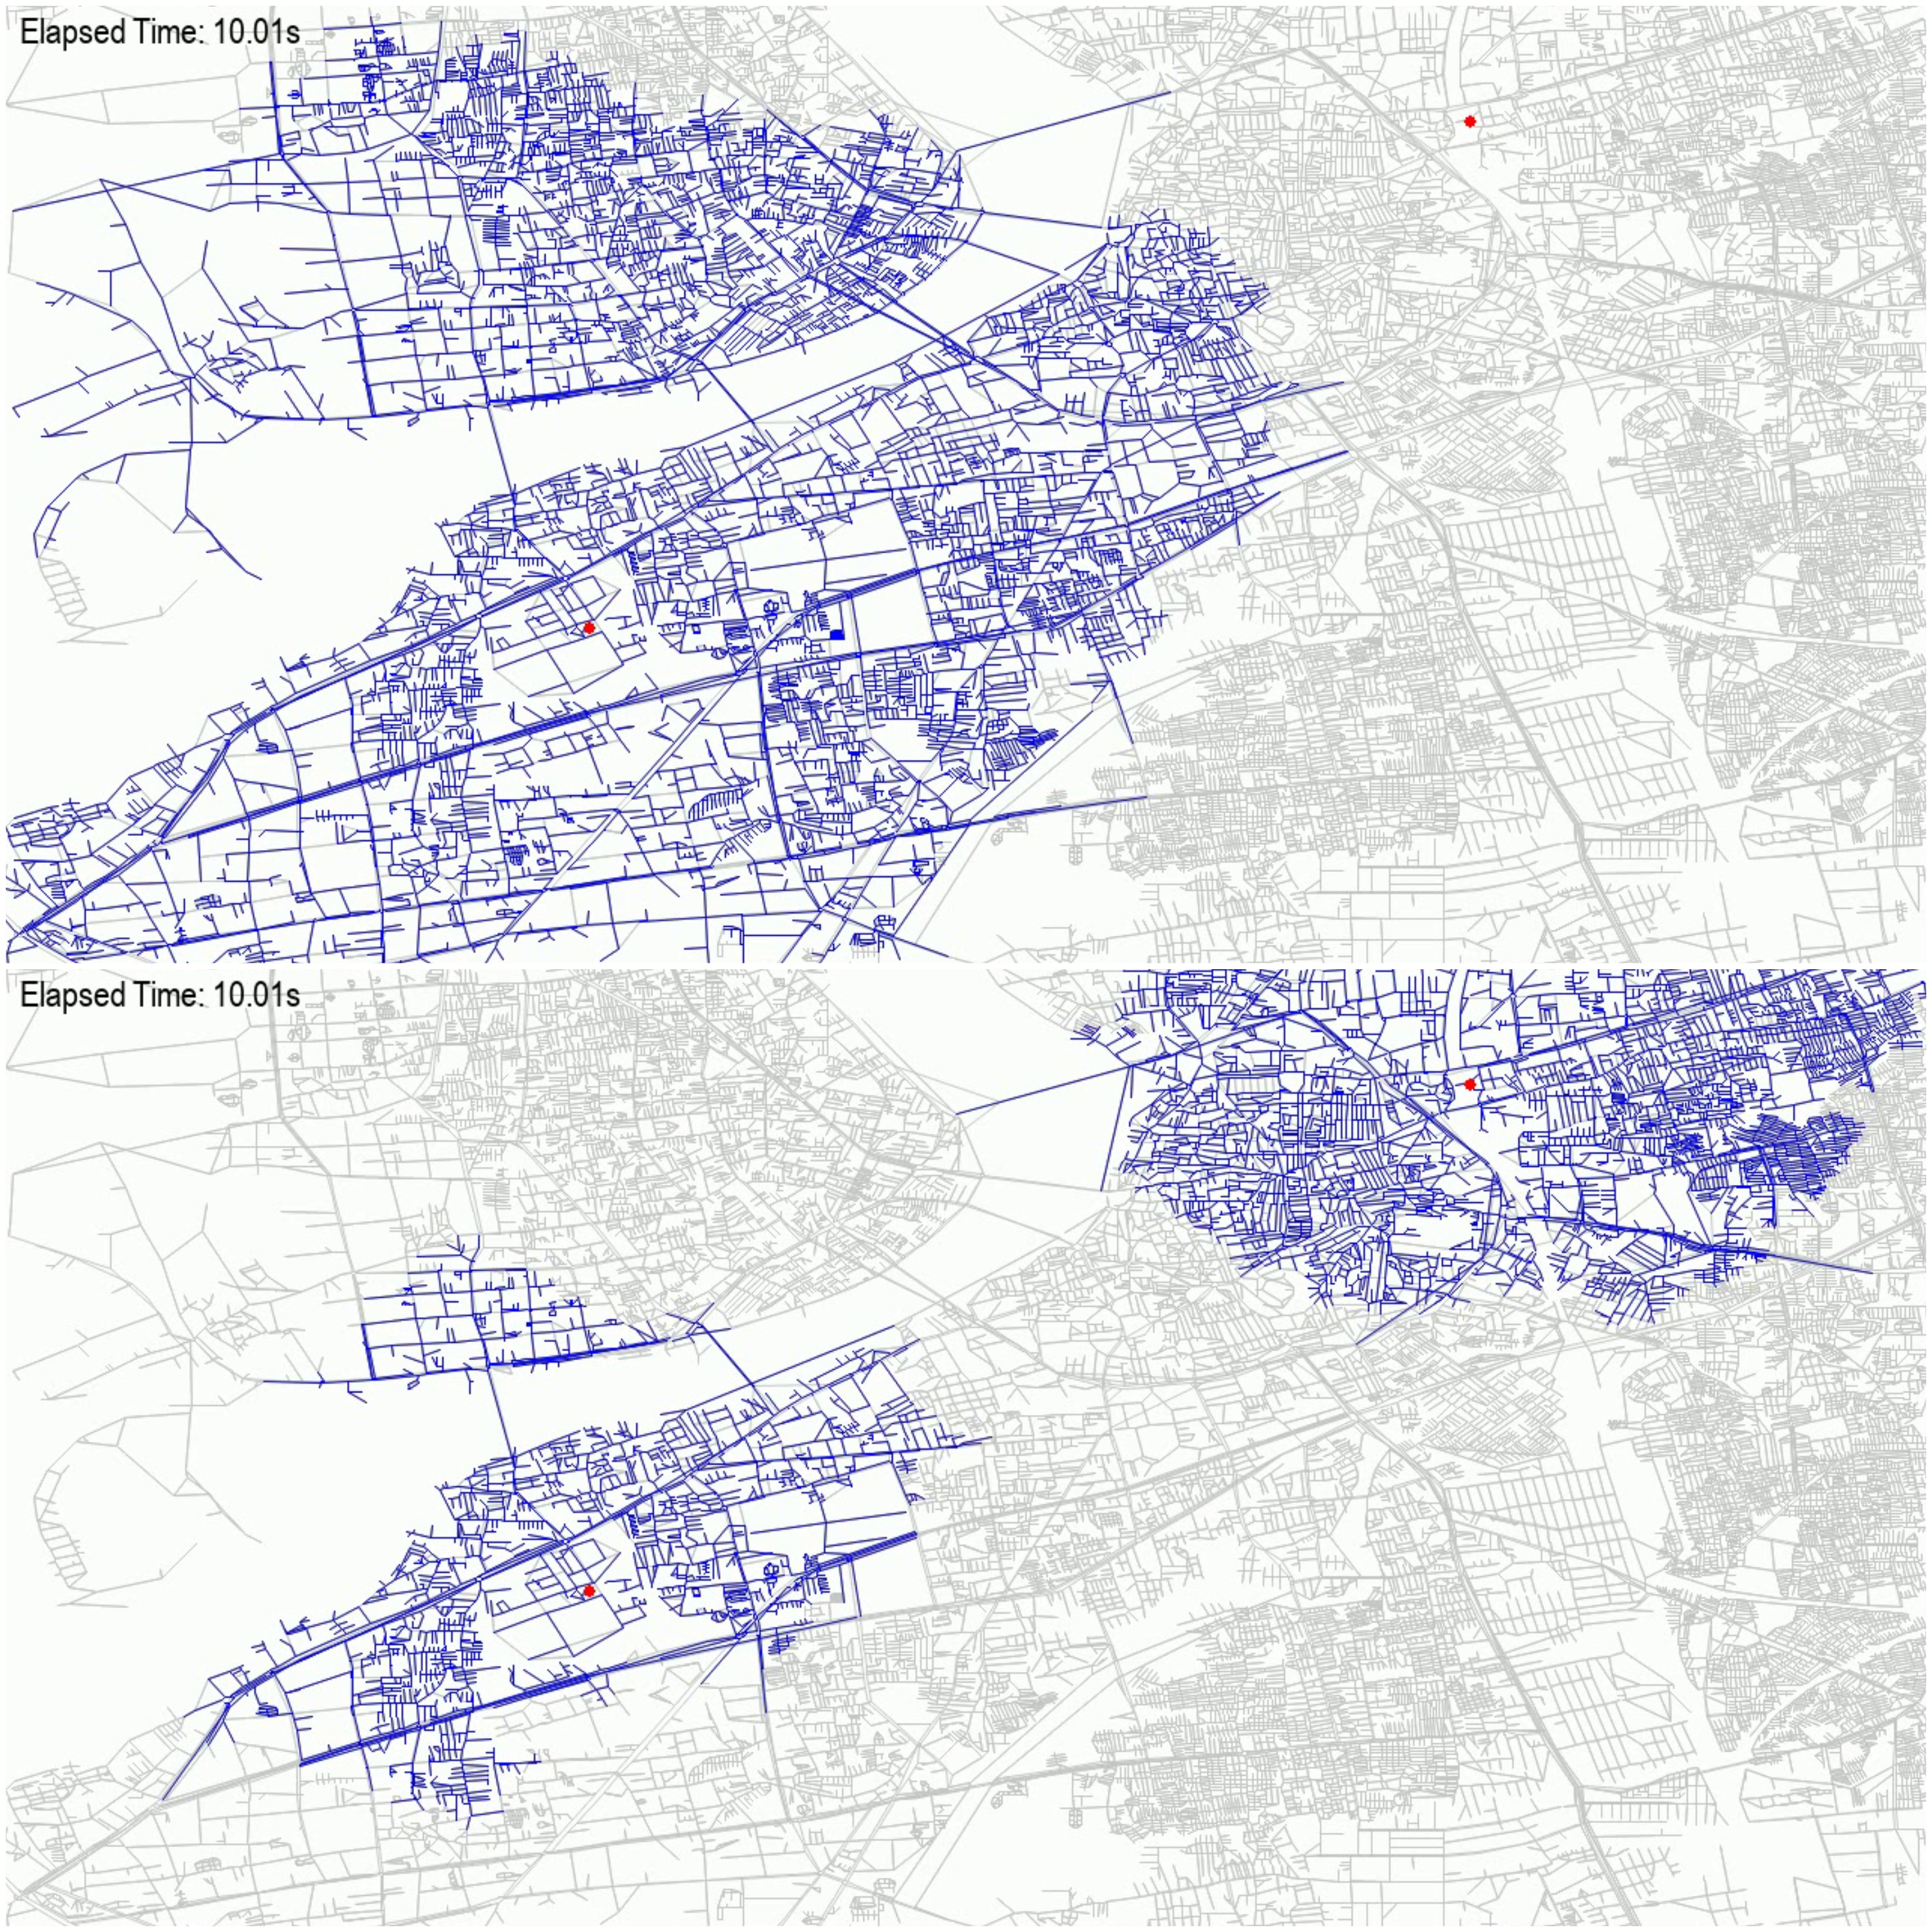
\includegraphics[width=0.7\textwidth]{astar_vs_bidijkstra.png}
		 	\caption{Visualization of explored edges at $t$ $=$ $10s$ for Version 2 (A* search) vs Version 3 (Bidirectional Dijkstra's).}
		 	\label{fig:bidirectional_dijkstra_vs_astar}
		 \end{figure}

		 While this version employs a less sophisticated path exploration strategy compared to the previous one, it achieves enhanced performance because bidirectional Dijkstra's algorithm can terminate as soon as the forward and backward searches meet. In contrast, A* continues until the target node is fully expanded, making its performance heavily dependent on the quality of the heuristic used.
	 
	 \section{Version 4: Bidirectional A* Search Algorithm}
	 	Running the timing code on this version produced the following output:
	 	\begin{verbatim}
	 		NetworkX time:  0.7203088998794556
	 		Algorithm time:  13.28147240029648
	 		NetworkX's algorithm takes 5.4234% of Algorithm's time
	 	\end{verbatim}
	 	
	 	This represents a \(\frac{4.1934}{3.5578} \approx 1.18\times\) improvement over Version 3. \newline \vspace{4mm}
	 	
	 	The enhanced performance in this version stems from integrating the strengths of the previous two: employing a heuristic to guide path exploration and reducing the search space through bidirectional search.
	 
	 \section{Final Version: Bidirectional A* Search with ALT Preprocessing}
	 	Running the timing code on this version produced the following output:
	 	\begin{verbatim}
	 		NetworkX time:  0.6841806997545063
	 		Algorithm time:  4.040331699885428
	 		NetworkX's algorithm takes 16.9338% of Algorithm's time
	 	\end{verbatim}
	 	
	 	This represents a \(\frac{5.4234}{16.9338} \approx 3.12\times\) improvement in execution time compared to Version 4. \vspace{4mm}
	 	
	 	The substantial performance enhancement in this version is due to the integration of bidirectional A* search with the ALT preprocessing technique. By precomputing distances to strategically chosen landmarks, the ALT method provides more accurate heuristic estimates, effectively reducing the search space during query execution.\vspace{4mm}
	 	
	 	Although the preprocessing phase requires a non-trivial amount of time, this upfront cost is amortized over numerous queries, resulting in significantly faster average query responses. This approach is particularly beneficial in large-scale road networks, where rapid query times are essential.
	 	
	 	\begin{figure}[H]
	 		\centering
	 		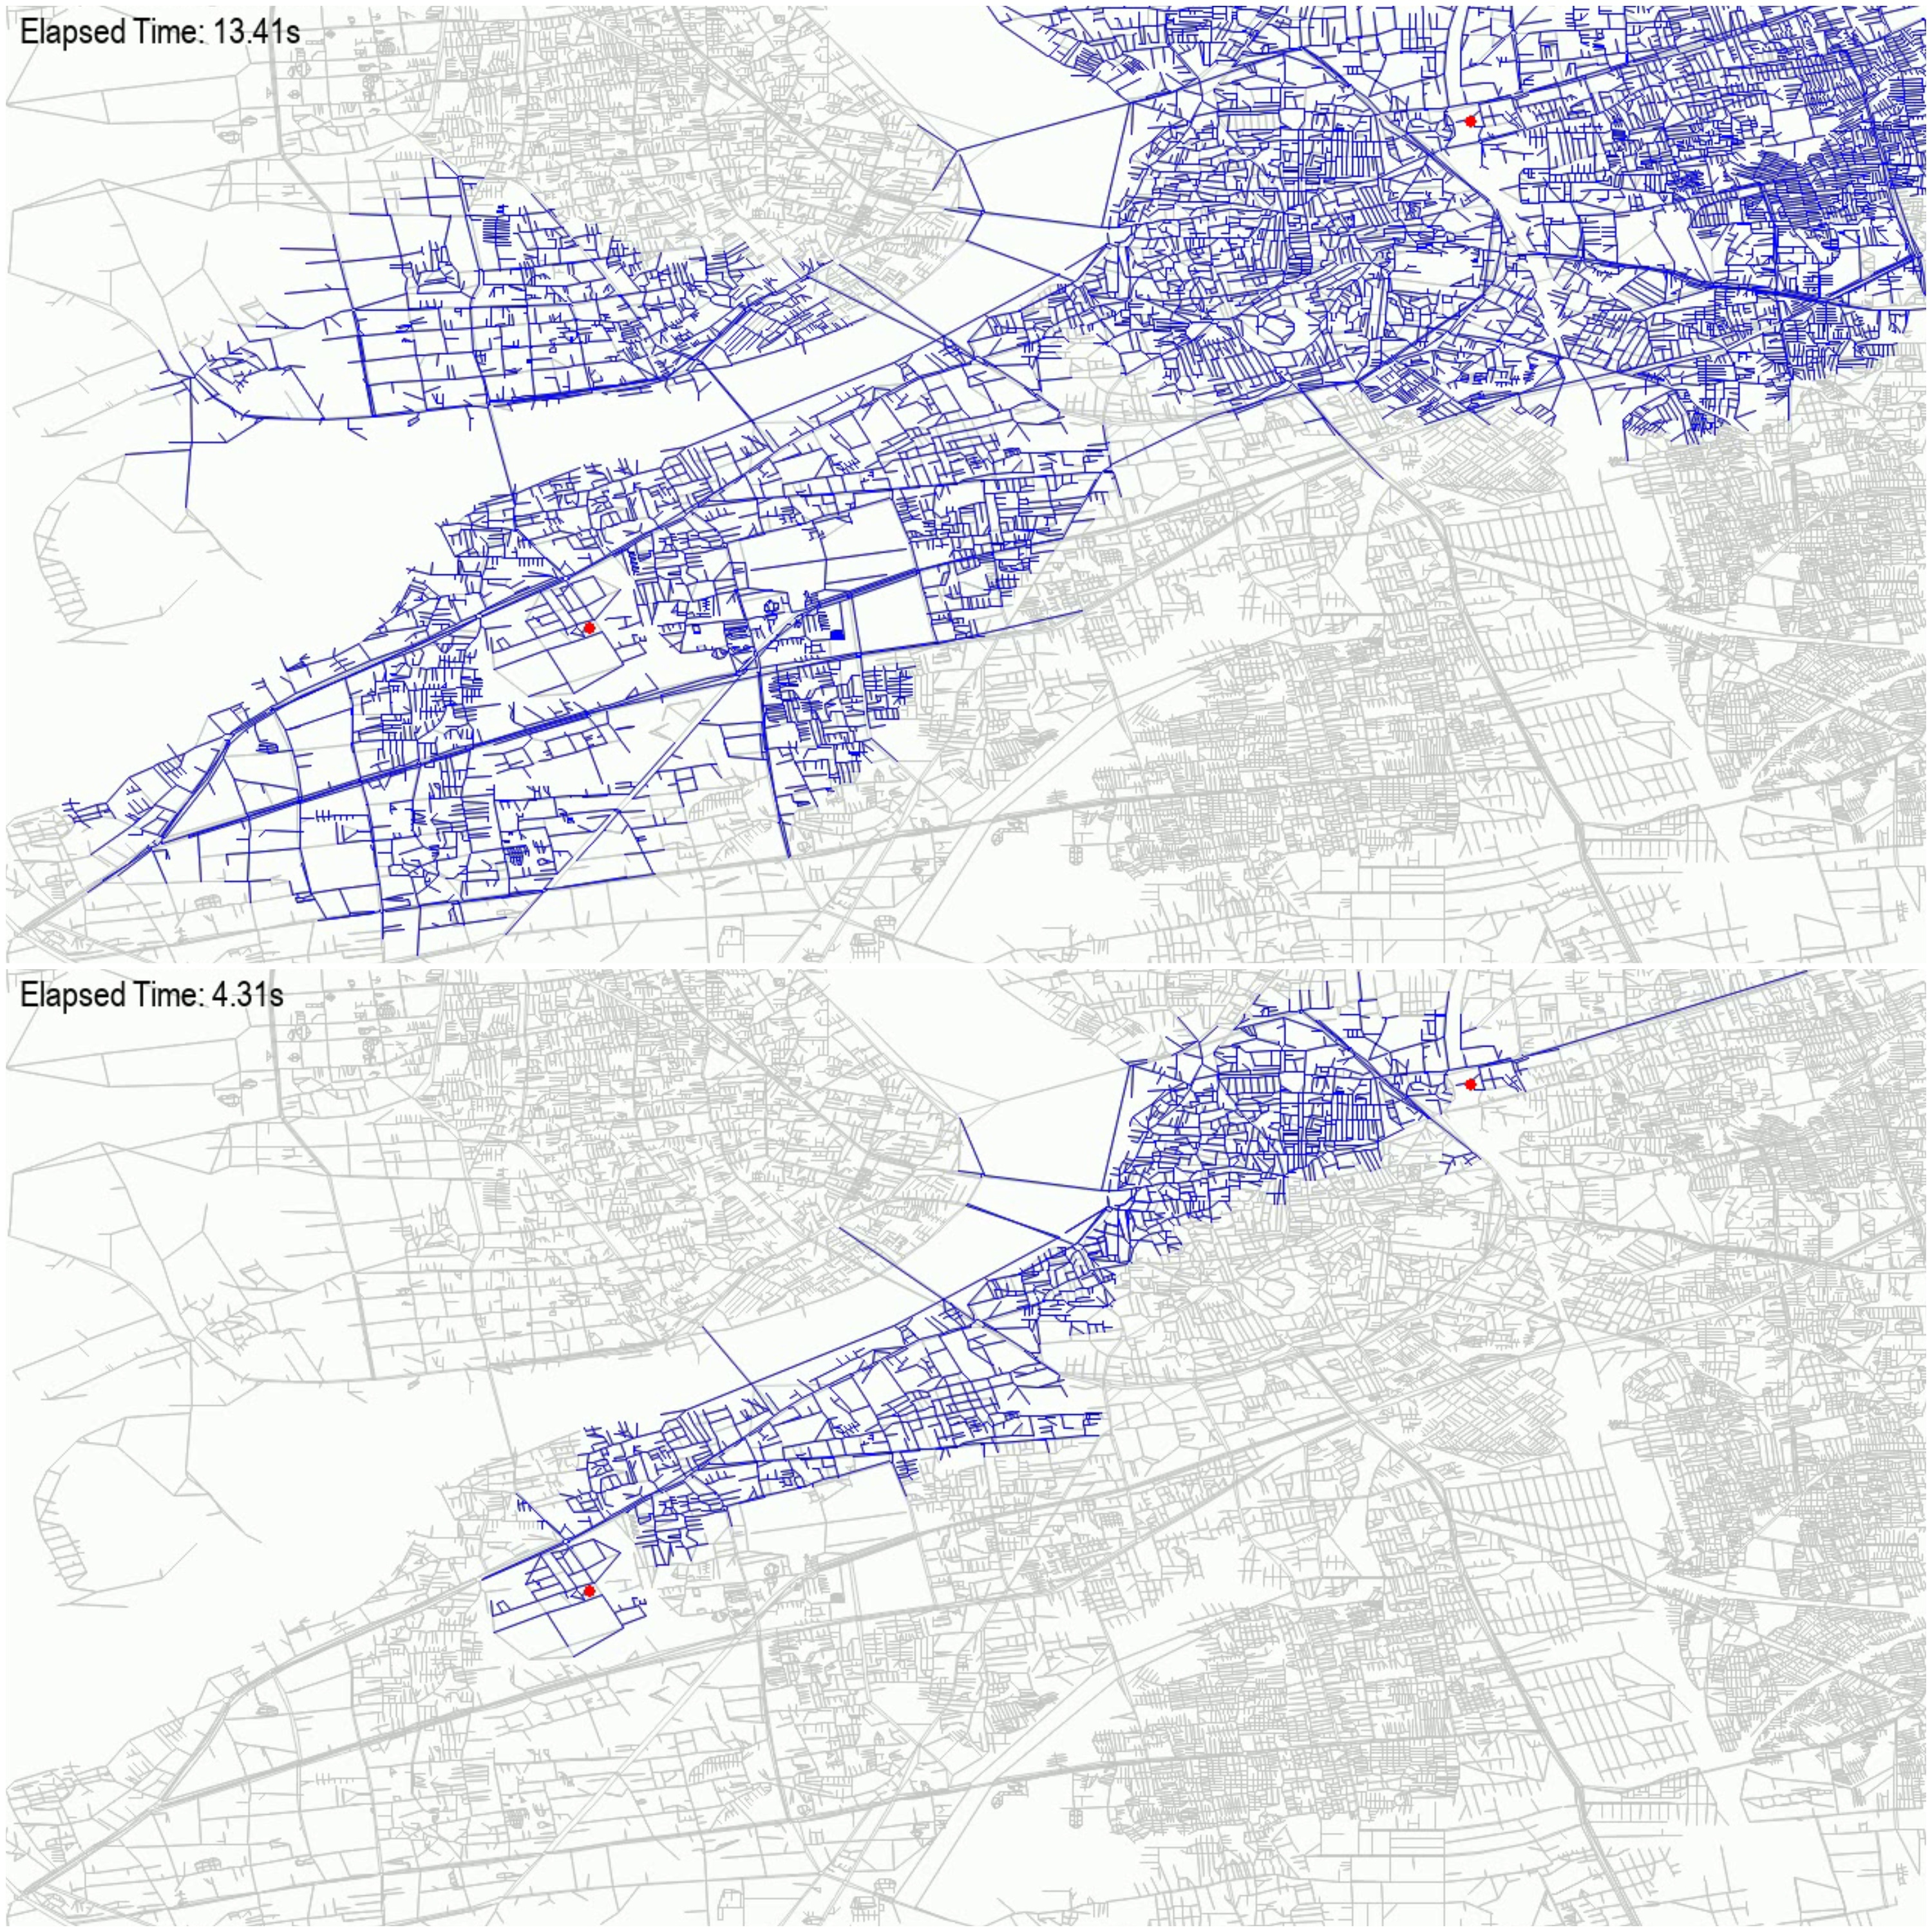
\includegraphics[width=0.7\textwidth]{final_vs_biastar.png}
	 		\caption{Visualization of all the explored edges in Version 4 (Bidirectional A*) vs Final Version (ALT + Bidirectional A*).}
	 		\label{fig:bidirectional_astar_vs_final}
	 	\end{figure}
	 	
	 	To get a more concrete comparison of the final version of our algorithm against NetworkX's we use the following code which compares their performances over multiple randomly selected source-destination pairs. The process is broken down into several steps:
	 		
	 		\begin{enumerate}
	 			\item \textbf{Generating random source-destination pairs} and storing them in a list:
	 			\begin{lstlisting}
	 				nodes_list = list(G.nodes)
	 				sources_dests = list()
	 				for i in range(0, 100):
	 				sources_dests.append( {"source": random.choice(nodes_list),
	 					"dest": random.choice(nodes_list)} )
	 			\end{lstlisting}
	 			
	 			\item \textbf{Preprocessing the graph}:
	 			\begin{lstlisting}
	 				preprocessor = ALTPreprocessor(G)
	 			\end{lstlisting}

	 			\item \textbf{Comparing execution times} using the scheme used previously, i.e. taking the minimum of a $100$ runs:
	 			\begin{lstlisting}
	 				def compare_times(graph, source, dest):
	 				timer = timeit.Timer(lambda: nx.shortest_path(graph, source, dest, weight='length'))
	 				nx_time = min(timer.repeat(5, 100))
	 				
	 				timer = timeit.Timer(lambda: bidirectional_alt_query(graph, source, dest, preprocessor))
	 				algo_time = min(timer.repeat(5, 100))
	 				
	 				return nx_time / algo_time * 100
	 			\end{lstlisting}
	 			
	 			\item \textbf{Aggregating results} by iterating over all the generated source-destination pairs and storing them in a list, and then taking the mean of these results:
	 			\begin{lstlisting}
	 				percentanges = list()
	 				for source_dest in sources_dests:
	 				try:
	 				percentanges.append(compare_times(G, source_dest["source"], source_dest["dest"]))
	 				except:
	 				nx.exception.NetworkXNoPath
	 				
	 				mean_percentage = sum(percentanges) / len(percentanges)
	 				print(f"NetworkX's algorithm takes {mean_percentage:.4f} of Algorithm's time")
	 			\end{lstlisting}
	 		\end{enumerate}
	 	Here is the output from this test:
	 	\begin{verbatim}
	 		NetworkX's algorithm takes 196.4728% of Algorithm's time
	 	\end{verbatim}
	 	Which means our algorithm is $\approx 2\times$ faster than NetworkX's \texttt{shortest\_path} implementation on average. This is expected because NetworkX uses Dijkstra's algorithm by default. In the 'SVNIT $\to$ Surat Railway Station' route, the benefits of preprocessing are minimal compared to a plain Dijkstra's search, making it an edge case for our enhancements.
	 
\chapter{Discussion}

\section{Strengths}
	\begin{itemize}
		\item Highlight significant improvements in speed, accuracy, or flexibility.
		\item Discuss adaptability to various real-world scenarios.
	\end{itemize}
\section{Limitations}
	\begin{itemize}
		\item Discuss preprocessing overhead or constraints in memory usage.
		\item Identify scenarios where the hybrid approach might underperform.
	\end{itemize}
\section{Further Improvements}
	\begin{itemize}
		\item Enhancing scalability for distributed systems.
		\item Incorporating machine learning to predict edge weights dynamically.
		\item Extending to multimodal routing or 3D graphs.
	\end{itemize}
\chapter{Conclusion}


Optimizing shortest path calculations is crucial for efficient resource management across systems like navigation and network routing. Advanced pathfinding algorithms were developed and analyzed, with a strong emphasis on performance improvements through strategic preprocessing and hybrid query execution.  \\ \medskip

A thorough exploration of classical methods such as Dijkstra’s and Bellman-Ford extended to advanced techniques like A* and Bidirectional Search, along with preprocessing methods - Contraction Hierarchies, ALT, and Hub Labeling - that precomputed critical path data to accelerate queries. A hybrid algorithm integrating ALT preprocessing with bidirectional A* was designed for optimized execution. Strategic landmark selection and distance precomputation via the ALT Preprocessor streamlined the graph, enhancing heuristic accuracy and query efficiency. \\ \medskip

Efficient implementation was ensured through \texttt{networkx} and \texttt{heapq}, while a \texttt{pygame} based visualization tool provided interactive analysis, validating improvements in execution time and reliability.  \\ \medskip

Each algorithmic enhancement yielded improvements, with the final hybrid model—integrating ALT preprocessing with Bidirectional A*—outperforming standard NetworkX implementations by approximately 2x on average for random queries. \\ \medskip

Further improvements will incorporate real-time graph updates, time-dependent edge weights, support multimodal paths, enable large-scale deployment, and extend scalability to graphs with billions of nodes.  \\ \medskip

Integrating advanced pathfinding with preprocessing significantly improved performance and scalability. The hybrid algorithm strengthens efficiency in large-scale systems, offering a foundation for future advancements in shortest path calculations and their real-world applications.

\cleardoublepage
%\pagebreak
\phantomsection
\addcontentsline{toc}{chapter}{References}
\begin{thebibliography}{99}

\bibitem{citation-1-name-here}Cite all academic papers, libraries, datasets, and tools used. \url{<url here>}

\end{thebibliography}

\cleardoublepage
%\pagebreak
\phantomsection
\begin{appendices}
	\chapter{}
	\section{Proof of correctness for BFS}\label{appendix:bfs:correctness}
		We'll prove the correctness of BFS using mathematical induction.
		\begin{itemize}
			\item \textit{Inductive hypothesis}: For all nodes at distance
			$k$ from the source, BFS correctly computes $distance[v] = k$.
			\item \textit{Base case}: The source node $s$ has $distance[s] = 0$.
			\item \textit{Induction step}: Assume the hypothesis is true for nodes at a distance $k$ from $s$. Then their neighbours (nodes at distance $k + 1$) are enqueued and assigned $distance = k + 1$ before any nodes at $distance > k + 1$ are processed.
			\item \textit{Conclusion}: BFS computes the shortest possible path for all reachable nodes.
		\end{itemize}
	\section{Proof of complexity for BFS}\label{appendix:bfs:complexity}
		Let us assume a graph $G(V, E)$ with $V$ vertices and $E$ edges.
	\begin{itemize}
		\item Mark all $V$ vertices as unvisited. This takes $O(V)$ time.
		\item Each vertex enters the queue once (when discovered) and exits the queue once. Enqueue and dequeue operations are $O(1)$, so processing all vertices takes $O(V)$ time.
		\item For each dequeued vertex $u$, iterate through its adjacency list to check all edges $(u,v)$.
		\item In a directed graph, each edge $(u,v)$ is processed once. In an undirected graph, each edge $(u,v)$ is stored twice (once for $u$ and once for $v$), but each is still processed once during BFS.
		\item Summing over all vertices, the total edge-processing time is $O(E)$.
	\end{itemize}
		Thus, the overall time complexity is $O(V+E)$.
	\section{Proof of correctness for Bellman-Ford}\label{appendix:bellford:correctness}
	We'll prove the correctness of Bellman-Ford algorithm using mathematical induction.
	\begin{itemize}
		\item \textit{Inductive hypothesis}: After $k$ iterations, $distance[v]$ is the length of the shortest path from $s$ to $v$ using at most $k$ edges.
		\item \textit{Base case}: After 0 iterations, $distance[s]=0$ (correct), and $distance[v] = \infty$ for all $v \neq s$ (no paths have been explored yet).
		\item \textit{Induction step}: Consider the $(k+1)^{th}$ iteration. For each edge $(u,v)$, if $distance[u]+w(u,v)<distance[v]$, then $distance[v]$ is updated to $distance[u]+w(u,v)$. This ensures that after $k+1$ iterations, $distance[v]$ is the length of the shortest path using at most $k+1$ edges.
		\item \textit{Conclusion}: After $V-1$ iterations, all shortest paths with at most $V-1$ edges have been found. Since a shortest path in a graph with $V$ vertices cannot have more than $V-1$ edges, the algorithm is correct.
		\item \textit{Negative cycle detection}: After $V - 1$ iterations, if any $distance[v]$ can still be improved (i.e. $distance[u]+w(u,v)<distance[v]$ for some edge $(u,v)$), then the graph contains a negative-weight cycle reachable from $s$.
	\end{itemize}
	\section{Proof of complexity for Bellman-Ford}\label{appendix:bellford:complexity}
	Let us assume a graph $G(V, E)$ with $V$ vertices and $E$ edges.
	\begin{itemize}
		\item Set $distance[s]=0$ and $distance[v]=\infty$ for all $v \neq s$. This takes $O(V)$ time.
		\item Relax all $E$ edges, repeated $V - 1$ times. Each relaxation takes $O(1)$ time. This takes a total time of $O(V \cdot E)$.
		\item For negative cycle detection, relax all the edges once more. This takes $O(E)$ time.
	\end{itemize}
	The dominant term is the relaxation step, which takes $O(V \cdot E)$ time, hence the overall complexity of the algorithm is $O(V \cdot E)$.
	\section{Proof of correctness for Dijkstra's}\label{appendix:dijkstra:correctness}
	We'll prove the correctness of Dijkstra's algorithm using mathematical induction.
	\begin{itemize}
		\item \textit{Inductive hypothesis}: After $k$ vertices are extracted from $Q$, their distance distance values are the correct shortest path distances from $s$.
		\item \textit{Base case}: Initially, $distance[s]=0$ (correct), and $distance[v]=\infty$ for all $v \neq s$ (no paths have been explored yet).
		\item \textit{Induction step}: Let $u$ be the $(k+1)^{th}$ vertex extracted from $Q$. Suppose there exists a shorter path to $u$ not using the extracted vertices. This path must leave the set of extracted vertices at some edge $(x,y)$, but since $w(x,y) \geq 0$, this would imply $distance[y]<distance[u]$, contradicting $u$’s extraction.
		\item \textit{Conclusion}: After all vertices are processed, the $distance$ array contains the correct shortest path distances.
	\end{itemize}
	\section{Proof of complexity for Dijkstra's}\label{appendix:dijkstra:complexity}
	Let us assume a graph $G(V, E)$ with $V$ vertices and $E$ edges. In a priority-queue based implementation of the algorithm,
	\begin{itemize}
		\item Each vertex is extracted once ($V \times \mbox{Extract-Min})$ and each edge is relaxed once $(E \times \mbox{Decrease-Key})$.
		\item Extract-Min and Decrease-Key take $O(\log{V})$ time in a binary heap.
		\item Extract-Min and Decrease-Key take $O(\log{V})$ and $O(1)$ time respectively in a fibonacci heap.
		\item For a binary heap, $V \times \mbox{Extract-Min}$ takes $O(V\log{V})$ time and $E \times \mbox{Decrease-Key}$ takes $O(E\log{V})$ time $\to$ a total complexity of $O((V + E)\log{V})$
		\item For a fibonacci heap, $V \times \mbox{Extract-Min}$ takes $O(V\log{V})$ time and $E \times \mbox{Decrease-Key}$ takes $O(E)$ time $\to$ a total complexity of $O(V\log{V} + E)$.
	\end{itemize}
	\section{Proof of correctness for A* search}\label{appendix:astar:correctness}
	We'll prove the correctness of A* search algorithm using mathematical induction. Let us define the following: \\
	$f(s)$: Estimated total cost of the path from the start node to the goal node, passing through the current node. \\
	$g(s)$: Cost of the shortest path from the start node to the current node. \\
	$h(s)$: Heuristic estimate of the cost from the current node to the goal node.
	\begin{itemize}
		\item \textit{Inductive hypothesis}: At each step, the node $u$ with the smallest $f(u)$ is the one with the smallest estimated total cost to the goal.
		\item \textit{Base case}: Initially, $g(s)=0$ and $f(s)=h(s)$. The start node $s$ is correctly prioritized.
		\item \textit{Induction step}: 
			\begin{itemize}
				\item When $u$ is extracted, its $g(u)$ is the true shortest path cost from $s$ to $u$ (due to admissibility and consistency).
				\item For each neighbor $v$, $f(v)=g(v)+h(v)$ is updated to reflect the best-known path to $v$.
				\item The algorithm continues to explore nodes in order of increasing $f(v)$, ensuring the shortest path is found.
			\end{itemize}
		\item \textit{Conclusion}: If the goal $t$ is reached, $g(t)$ is the true shortest path cost and If $Q$ becomes empty, no path exists.
	\end{itemize}

\section{Proof of correctness for ALT}\label{appendix:ALT:correctness}

\begin{itemize}
	\item Admissibility of $h(v)$: A heuristic is admissible if it never overestimates the true distance:  
	\begin{equation*} h(v) \leq d(v, t) \end{equation*}
	By the \textit{triangle inequality}: \begin{equation*} d(v, t) \geq |d(L, v) - d(L, t)| \quad \forall L \in L \end{equation*}
	Taking the maximum over all landmarks:
	\begin{equation*}
		d(v, t) \geq \max_{L \in \textit{L}} \left| d(L, v) - d(L, t) \right| = h(v)
	\end{equation*}
	Thus, $ h(v) $ is admissible.
	\item Consistency of $h(v)$: A heuristic is consistent if for any edge $ (u, v) $:
	\begin{equation*}
		h(v) \leq d(u, v) + h(u)
	\end{equation*}
	Using the \textit{triangle inequality}:
	\begin{equation*} 
		|d(L, v) - d(L, t)| \leq d(u, v) + |d(L, u) - d(L, t)| 
	\end{equation*}
	Taking the maximum over all landmarks:
	\begin{equation*}
		h(v) = \max_{L \in \textit{L}} \left| d(L, v) - d(L, t) \right| \leq d(u, v) + h(u)
	\end{equation*}
	Thus, $ h(v) $ is consistent.
\end{itemize}
Since $ h(v) $ is both admissible and consistent, the ALT algorithm guarantees optimal shortest paths.

\section{Proof of complexity for ALT}\label{appendix:ALT:complexity}
	\begin{itemize}
		\item Landmark Selection:
			\begin{itemize}
				\item \textit{Randomly selecting landmarks}: This is a constant-time operation, $ O(1) $.
				\item \textit{Selecting high-degree or far-apart nodes}: This might involve sorting the nodes based on degree or distance, which would take $ O(|V| \log |V|) $, where $ |V| $ is the number of nodes in the graph.
			\end{itemize}
		\item Precompute Shortest Path Distances from Landmarks: For $k$ landmarks, we need to perform Dijkstra’s algorithm $k$ times, one for each landmark, making the total preprocessing time complexity is $O(k \cdot (|V| + |E|) \log |V|)$.
		\item Query Phase Complexity: The A* search algorithm with ALT uses the ALT heuristic $ h(v) $ instead of a simple heuristic (like Euclidean distance). The time complexity of the A* search depends on the number of nodes expanded during the search and the priority queue operations. In the worst case, the complexity is $ O((|V| + |E|) \log |V|) $. The average query time is generally much faster, but it is difficult to bound precisely without empirical data.		
	\end{itemize}

\section{Proof of correctness for Hub Labellling}\label{appendix:Hub Labelling:correctness}
	\begin{itemize}
		\item During the preprocessing phase of the Hub Labeling algorithm, we ensure that for any pair of nodes $ u $ and $ v $, their labels $ L(u) $ and $ L(v) $ share at least one common hub $ h $ that lies on the shortest path between $ u $ and $ v $.
		\item Formally, for any two nodes $ u, v \in V $, there exists a hub $ h \in L(u) \cap L(v) $ such that $ h $ lies on the shortest path between $ u $ and $ v $, i.e., the path $ u \to h \to v $ is a valid shortest path. Thus, this \textit{Label Cover Property} ensures that the correct hubs are selected in the query phase and the algorithm can always compute the shortest path.
		\item For any two nodes $ u $ and $ v $, during the query phase, the algorithm scans their labels $ L(u) $ and  $ L(v) $ to find the hub $ h $ that minimizes the expression $ d(u, h) + d(h, v) $. This is equivalent to finding the shortest path between $ u $  and $ v $ by traversing through a common hub $ h $.
		\item Since $ h $ lies on the shortest path between $ u $ and $ v $ (by the Label Cover Property), the value $ d(u, h) + d(h, v) $ is guaranteed to be the shortest path distance between $ u $ and $ v $.
		\item Therefore, the Hub Labeling algorithm correctly computes the shortest path for any query $ (u, v) $, as it always finds the optimal hub $ h $ and ensures that the sum of distances $ d(u, h) + d(h, v) $ corresponds to the actual shortest path distance.
	\end{itemize}

\section{Proof of complexity for Hub Labelling}\label{appendix:Hub Labelling:Complexity}
	\begin{itemize}
		\item For each node $v$, compute the forward and backward labels using Dijkstra's algorithm or a similar shortest path algorithm.
		\item The time complexity for computing labels for all nodes is $O(V \cdot (V+E)\log V)$, where $V$ is the number of nodes and $E$ is the number of edges.
		\item The selection of hubs can be done using various strategies, such as selecting nodes with high centrality or using a greedy algorithm. The time complexity for hub selection is $O(VlogV)$.
		\item For a given query $(s,t)$, the forward label of $s$ and the backward label of $t$ are intersected to find the shortest path distance.
		\item The time complexity for label intersection is $O(|L_f(s)| + |L_b(t)|)$, where $|L_f(s)|$ and $|L_b(t)|$ are the sizes of the forward and backward labels, respectively.
		\item Each node stores a forward label and a backward label. The space complexity for storing all labels is $O(V \cdot L)$, where $L$ is the average label size.
	\end{itemize}
	
	
\end{appendices}

\end{document}
